\title{Assignment 1 \\ \small{Evolutionary Computing}}
\author{Chiel ten Brinke 3677133}
\documentclass[12pt]{article}
\usepackage{amssymb,amsmath,amsthm,enumerate,graphicx,float,lmodern,xparse}

\newtheorem{theorem}{Theorem}[section]
\newtheorem{lemma}[theorem]{Lemma}
\newtheorem{proposition}[theorem]{Proposition}
\newtheorem{corollary}[theorem]{Corollary}

\theoremstyle{definition}
\newtheorem{definition}[theorem]{Definition}
\newtheorem{axiom}[theorem]{Axiom}
\newtheorem{example}[theorem]{Example}
\newtheorem{remark}[theorem]{Remark}

\NewDocumentCommand\set{mg}{%
    \ensuremath{\left\lbrace #1 \IfNoValueTF{#2}{}{\, \middle|\, #2} \right\rbrace}%
}

\newcommand{\mytable}[3]{
\begin{table}[H]
\begin{tabular}{|ll|}
\hline
\textbf{Required population size} & #1            \\ \hline
\textbf{Function evaluations}     & #2            \\ \hline
\textbf{Corresponding CPU time}   & #3 seconds    \\ \hline
\end{tabular}
\end{table}
}

\begin{document}
\maketitle

\section*{Results}

\subsection*{Experiment 1}

\subsubsection*{Counting ones}
\mytable{310}{51094}{0.013}

\subsubsection*{Linearly scaled counting ones}
\mytable{730}{164174}{0.030}

\subsubsection*{Tightly linked deceptive trap}
\mytable{1210}{243142}{0.429}

\subsubsection*{Tightly linked non-deceptive trap}
\mytable{610}{93278}{0.177}


\begin{figure}[H]
    \centering
    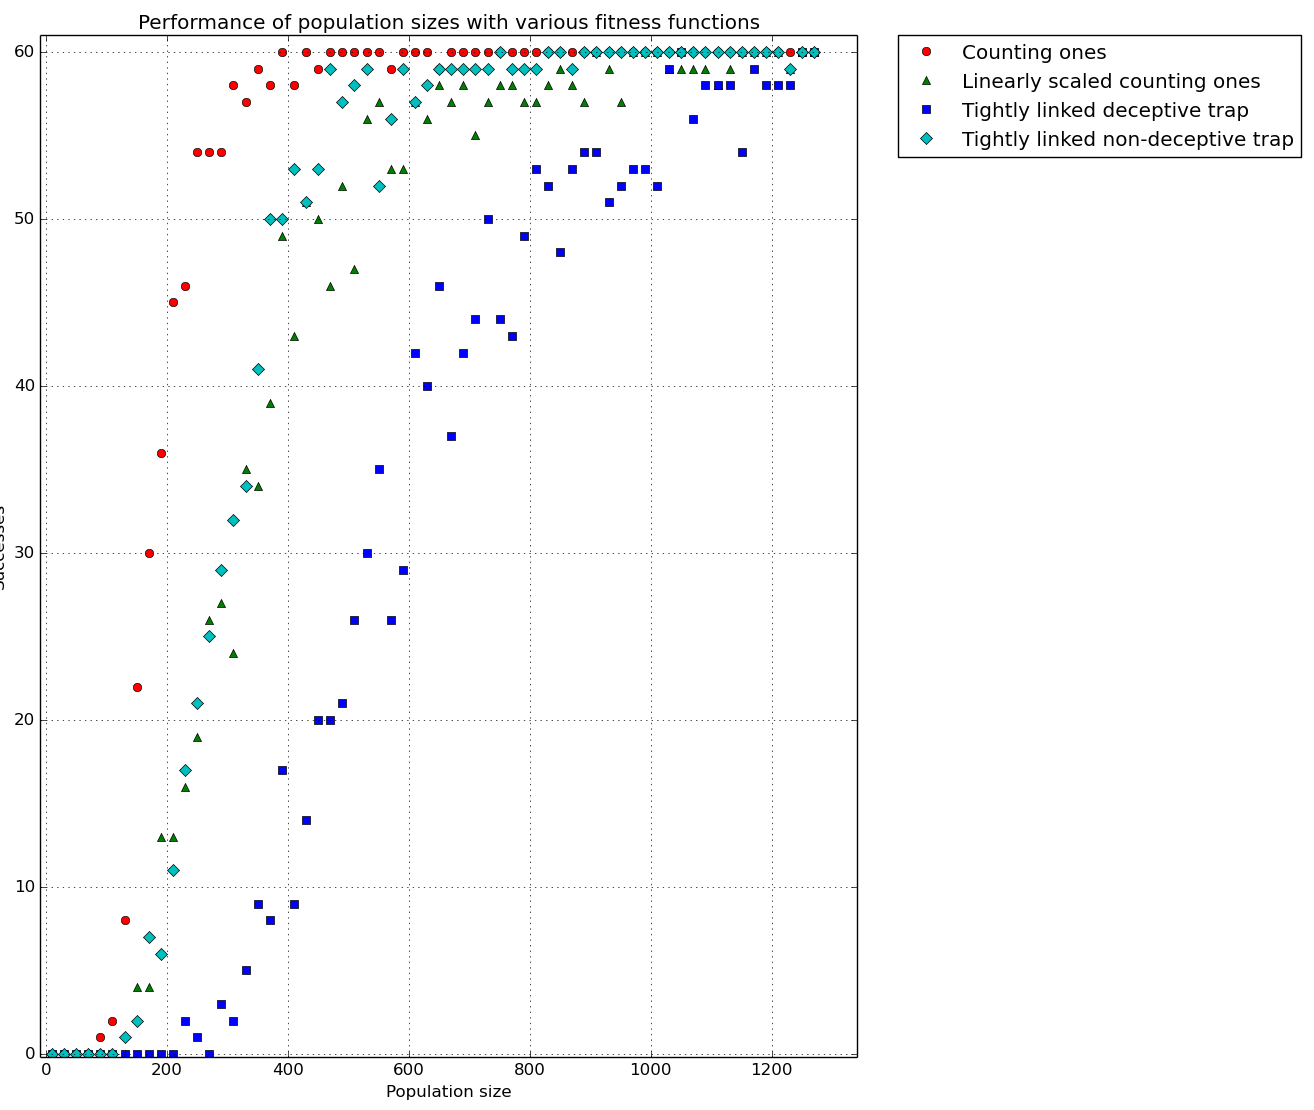
\includegraphics[width=1\linewidth]{images/exp1.png}
    \caption{TODO}
\label{fig:exp1}
\end{figure}


\subsection*{Experiment 2}

\subsubsection*{Counting ones}
\mytable{70}{9822}{0.002}

\subsubsection*{Linearly scaled counting ones}
\mytable{160}{28260}{0.005}

\subsubsection*{Tightly linked non-deceptive trap}
\mytable{850}{242154}{0.454}


\begin{figure}[H]
    \centering
    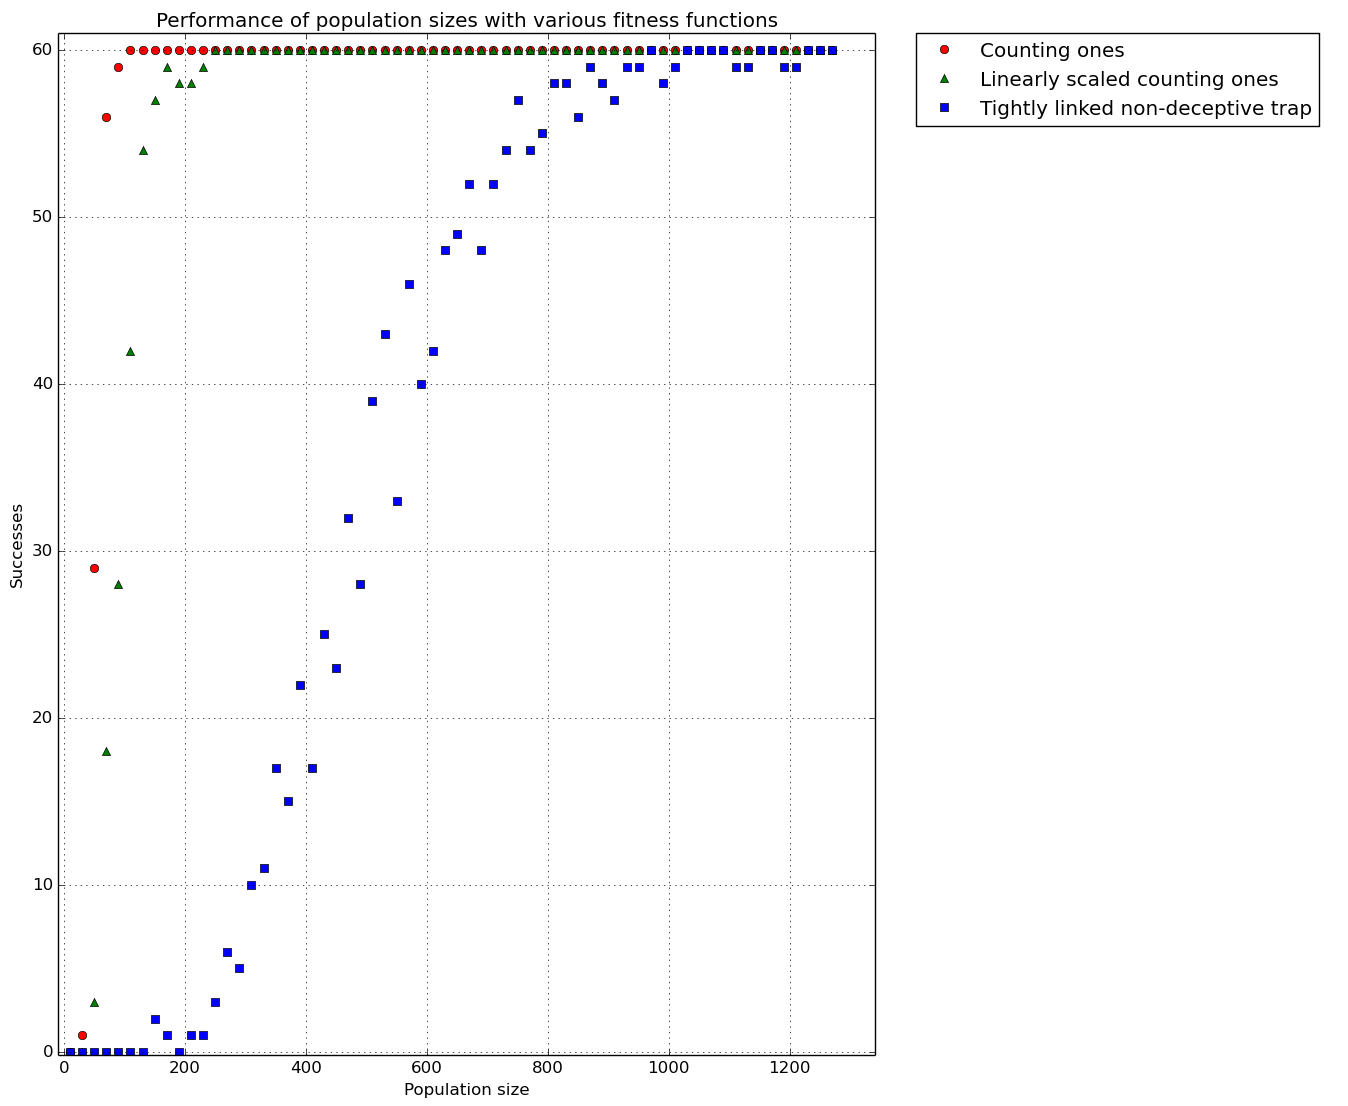
\includegraphics[width=1\linewidth]{images/exp2.png}
    \caption{TODO}
\label{fig:exp2}
\end{figure}


\subsection*{Experiment 3}

\subsubsection*{Counting ones}
\mytable{110}{27964}{0.007}

\subsubsection*{Linearly scaled counting ones}
\mytable{90}{49764}{0.010}

\subsubsection*{Tightly linked non-deceptive trap}
\mytable{490}{509742}{0.582}


\begin{figure}[H]
    \centering
    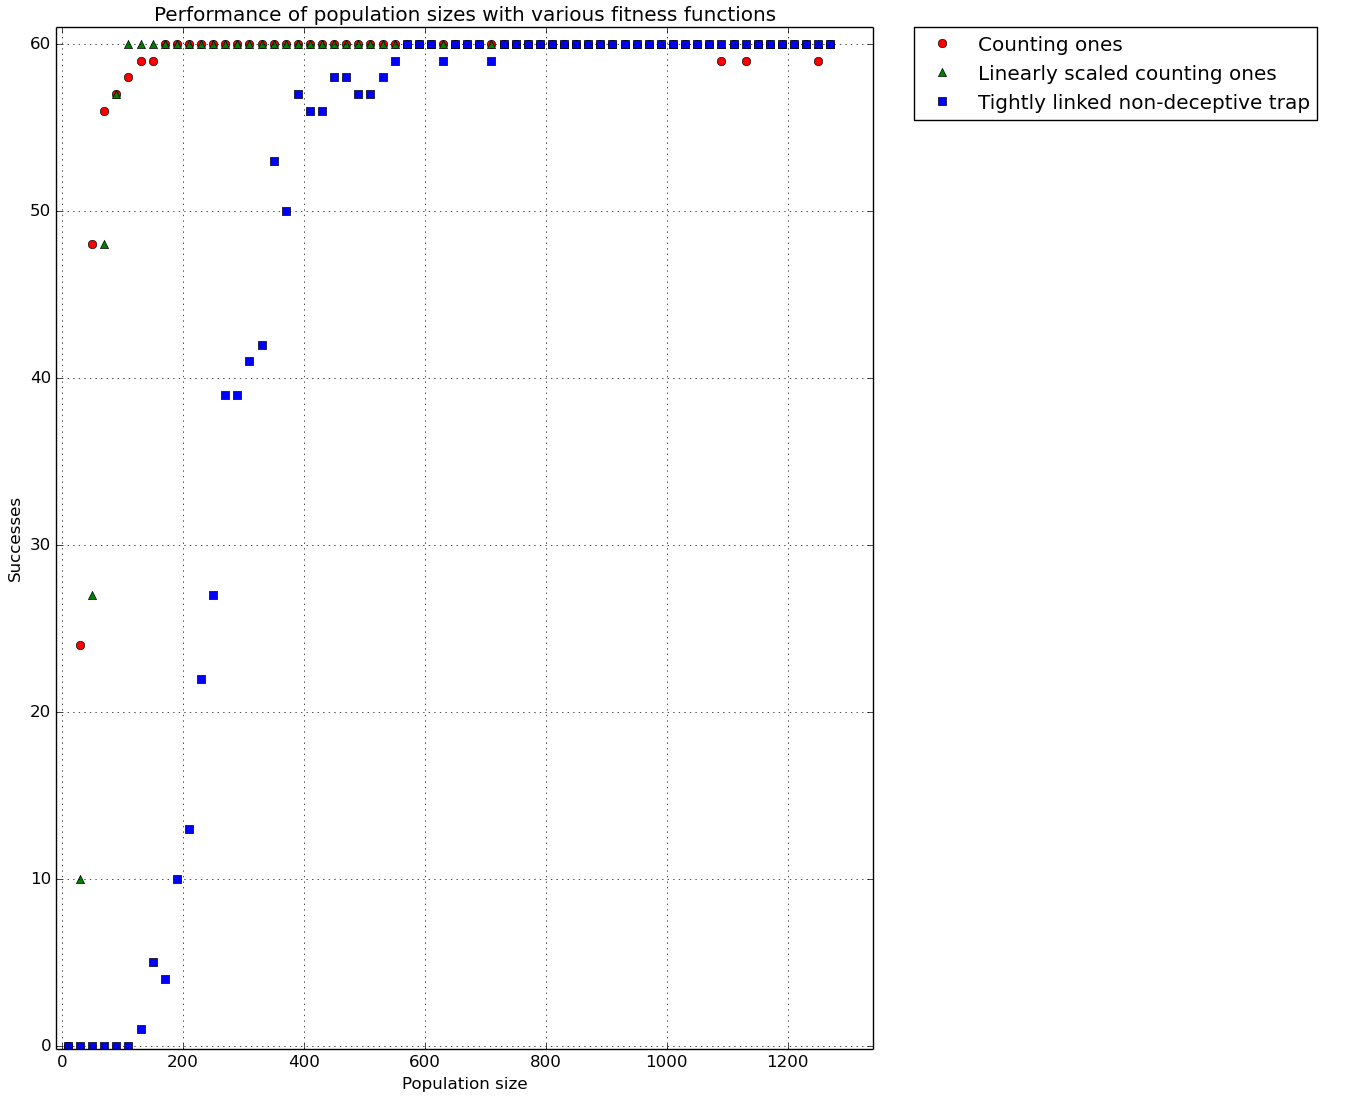
\includegraphics[width=1\linewidth]{images/exp3.png}
    \caption{TODO}
\label{fig:exp3}
\end{figure}

\end{document}
